\usetikzlibrary{3d,calc,backgrounds}

\pgfdeclarefunctionalshading{sphere}{\pgfpoint{-25bp}{-25bp}}{\pgfpoint{25bp}{25bp}}{}{
%% calculate unit coordinates
25 div exch
25 div exch
%% copy stack
2 copy 
%% compute -z^2 of the current position 
dup mul exch
dup mul add
1.0 sub
%% and the -z^2 of the light source 
0.3 dup mul
-0.5 dup mul add
1.0 sub
%% now their sqrt product
mul abs sqrt
%% and the sum product of the rest
exch 0.3 mul add
exch -0.5 mul add
%% max(dotprod,0)
dup abs add 2.0 div 
%% matte-ify
0.6 mul 0.4 add
%% currently there is just one number in the stack.
%% we need three corresponding to the RGB values
dup
0.4
}

\definecolor{verde}{HTML}{adda79}
\definecolor{naranjo}{HTML}{f38d70}

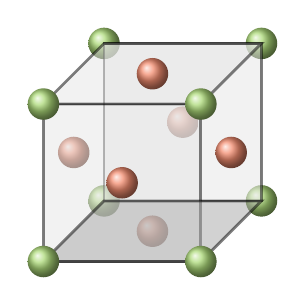
\begin{tikzpicture}[line width=1pt]

  \pgfdeclarelayer{background}
  \pgfsetlayers{background,main}

  \begin{scope}[canvas is xy plane at z=0]
    \draw[fill=black!10,opacity=0.5] (0,0) -- (0:2) -- ([turn]90:2) -- ([turn]90:2) -- cycle;
  \end{scope}
  \begin{scope}[canvas is xy plane at z=2]
    \draw[fill=black!10,opacity=0.5] (0,0) -- (0:2) -- ([turn]90:2) -- ([turn]90:2) -- cycle;
  \end{scope}
  \begin{scope}[canvas is zx plane at y=0]
    \draw[fill=black!35,opacity=0.5] (0,0) coordinate (E) -- (0:2) coordinate (F) -- 
      ([turn]90:2) coordinate (G) -- ([turn]90:2) coordinate(H) -- cycle;
    \global\coordinate (GE) at (E);
    \global\coordinate (GF) at (F);
    \global\coordinate (GG) at (G);
    \global\coordinate (GH) at (H);
  \end{scope}
  \begin{scope}[canvas is zx plane at y=2]
    \draw[fill=black!10,opacity=0.5] (0,0) coordinate (A) -- (0:2) coordinate (B) -- 
      ([turn]90:2) coordinate (C) -- ([turn]90:2) coordinate (D) -- cycle;
    \global\coordinate (GA) at (A);
    \global\coordinate (GB) at (B);
    \global\coordinate (GC) at (C);
    \global\coordinate (GD) at (D);
  \end{scope}

  \shade[ball color=verde] (GC) circle [radius=2mm];
  \shade[ball color=verde] (GB) circle [radius=2mm];
  \shade[ball color=verde] (GF) circle [radius=2mm];
  \shade[ball color=verde] (GG) circle [radius=2mm];
  \shade[ball color=naranjo] ($(GA)!0.5!(GC)$) circle [radius=2mm];
  \shade[ball color=naranjo] ($(GB)!0.5!(GG)$) circle [radius=2mm];
  \shade[ball color=naranjo] ($(GC)!0.5!(GH)$) circle [radius=2mm];
  \begin{pgfonlayer}{background}
    \shade[ball color=verde] (GA) circle [radius=2mm];
    \shade[ball color=verde] (GD) circle [radius=2mm];
    \shade[ball color=verde] (GE) circle [radius=2mm];
    \shade[ball color=verde] (GH) circle [radius=2mm];
    
    
    \shade[ball color=naranjo] ($(GA)!0.5!(GF)$) circle [radius=2mm];
    \shade[ball color=naranjo] ($(GE)!0.5!(GG)$) circle [radius=2mm];
    \shade[ball color=naranjo] ($(GD)!0.5!(GE)$) circle [radius=2mm];

  \end{pgfonlayer}

\end{tikzpicture}
